\documentclass{beamer}
\usepackage{moreverb} % Needed to allow comments, and verbatimwrite
\usepackage{verbatim}
\usepackage{ifthen} % Conditionals
\usepackage{bm} % BoldMath
\usepackage[econtex]{optional}

\usepackage[scale=2]{ccicons}
\usepackage{minted}
\usepackage{amsmath}
\usepackage{float}
\usepackage{setspace}
\usepackage{tikz}
\usepackage{caption}
\usemintedstyle{trac}
%\usepackage{biblatex}
%\addbibresource{economics.bib}

% if the line below is uncommented, bullets are shown step by step; comment out to make printable version
\beamerdefaultoverlayspecification{<+->}

% These are options to the compiler that can be sent at the command line
% This permits one document to generate multiple slightly different variations of the slides
\newboolean{WithOverlays}
\setboolean{WithOverlays}{true}
\newboolean{IMFMacroModelConf}
\setboolean{IMFMacroModelConf}{false}
%\setboolean{IMFMacroModelConf}{true}
\newboolean{FRBTalk}
\setboolean{FRBTalk}{false}
%\setboolean{FRBTalk}{true}
\newboolean{LSETalk}
\setboolean{LSETalk}{false}
\setboolean{LSETalk}{true}
\usepackage{optional}
\opt{NoOverlays}{\setboolean{WithOverlays}{false}\beamerdefaultoverlayspecification{}}

\mode<presentation>
{
  \usetheme{Warsaw}
  % or ...
  \setbeamercovered{transparent}
}

% Write the body to be read for autogeneration of printable version with 4 slides per page and no overlays
\begin{verbatimwrite}{./HeteroMacro-Slides-body.tex} 
\opt{FromShell}{
\provideboolean{IMFMacroModelConf}
\setboolean{IMFMacroModelConf}{false}
\provideboolean{IMFMacroModelConf}
\setboolean{IMFMacroModelConf}{false}
\provideboolean{LSETalk}
\setboolean{LSETalk}{true}
\provideboolean{FRBTalk}
\setboolean{FRBTalk}{true}
}
\opt{IMFMacroModelConf}{\setboolean{IMFMacroModelConf}{true}}
\opt{LSETalk}{\setboolean{LSETalk}{true}}
\opt{FRBTalk}{\setboolean{FRBTalk}{true}}

\newcommand{\ifIMF}{\ifthenelse{\boolean{IMFMacroModelConf}}}
\newcommand{\ifFRB}{\ifthenelse{\boolean{FRBTalk}}}
\newcommand{\ifLSE}{\ifthenelse{\boolean{LSETalk}}}

\newboolean{HeteroMacro}
\setboolean{HeteroMacro}{true}

\usepackage{cancel}
\usepackage{econtexShortcuts}
%\newcommand{\newblock}{} % Needed to make beamer work with bibtex

\pdfmapfile{+sansmathaccent.map}
% Jirka's definitions
\usepackage{booktabs}
\usepackage{natbib}
%\usepackage{apalike}
\definecolor{jirkasred}{rgb}{0.9,0,0}
\newcommand{\jemph}[1]{{\color{jirkasred}#1}}
%\def\newblock{\hskip .11em plus .33em minus .07em}

\renewcommand{\ptyLev}{\ensuremath{Z}} % Z for productivity
\renewcommand{\urate}{\ensuremath{u}}
\renewcommand{\erate}{\ensuremath{\cancel{\urate}}}

%\setbeamertemplate{navigation symbols}{}  % Take away navigation symbols

%_____________ Opening slide _______________________

\title[HeteroMacro]{{New Perspectives on Consumption \\ Panel Discussion}}
\author[Carroll]{\scriptsize{Christopher Carroll\inst{1}}}

% - Use the \inst command only if there are several affiliations.
% - Keep it simple, no one is interested in your street address.
\institute{
  \inst{1} Johns Hopkins University and NBER\\   \texttt{ccarroll@jhu.edu} 
    }
\date{\today \\
\ifIMF{19th IMF Macro Modeling Conference \\ Armenia \\ September 2016}{}
\ifFRB{Presentation at Federal Reserve Board \\ September 2016 \\ Largely Based on \cite{cstwMPC} \\ {\small Thanks also to David Low, Nathan Palmer, and Alex Kaufman}}{}
\ifLSE{London School of Economics \\ December 2016}{}
}

\begin{document}

\begin{frame}[plain]
  \titlepage
\end{frame}


\begin{frame}\frametitle{Progress!}

\pause 
\bi
\item I feel the way Galileo must have felt ...
\item ... before he started grinding lenses
\item Conference shows lots of people grinding away!
\bi
\item National Registry Data (`Registries')
\item Administrative Data from Aggregators (`Aggregators')
\item Consumer Credit Panels (`CCP')
\item Surveys
\ei

\ei


\end{frame}

\begin{frame}\frametitle{What Would the Perfect Lens Look Like?}

Perfection:
\bi
\item Huge Sample Sizes 
\bi
\item (Registries; Aggregators)
\ei
\item Accurately Measured Data on $\cRat, \yRat, \aRat, \dRat$
\bi
\item (Registries; Aggregators)
\ei
\item Data on {\it expectations} and {\it preferences}
\bi
\item (Surveys)
\ei
\ei

What we most desperately need:
\bi
\item  {\it Integrated}: Balance sheets {\it and} expectations
\item Leth-Petersen is the only example (and small sample size)
\ei

\end{frame}


% \section{Why Do We Care?}
\begin{frame}\frametitle{Why Do We Care?}

\bi
\item Microeconomics
\bi 
\item Lots of reasons
\ei
\item Macroeconomics
\bi
\item ``Aggregate Demand''
%\item Capital Stock $\Rightarrow$ Interest Rates
\item Finance-Macro Nexus
\ei
\ei

\end{frame}

\begin{frame}\frametitle{Larry Summers' Infamous Quote about 2009-10}

{\it ``Almost nothing from the academic macroeconomics literature over the prior
30 years was useful in understanding what to do''} 


\begin{center}
\phantom{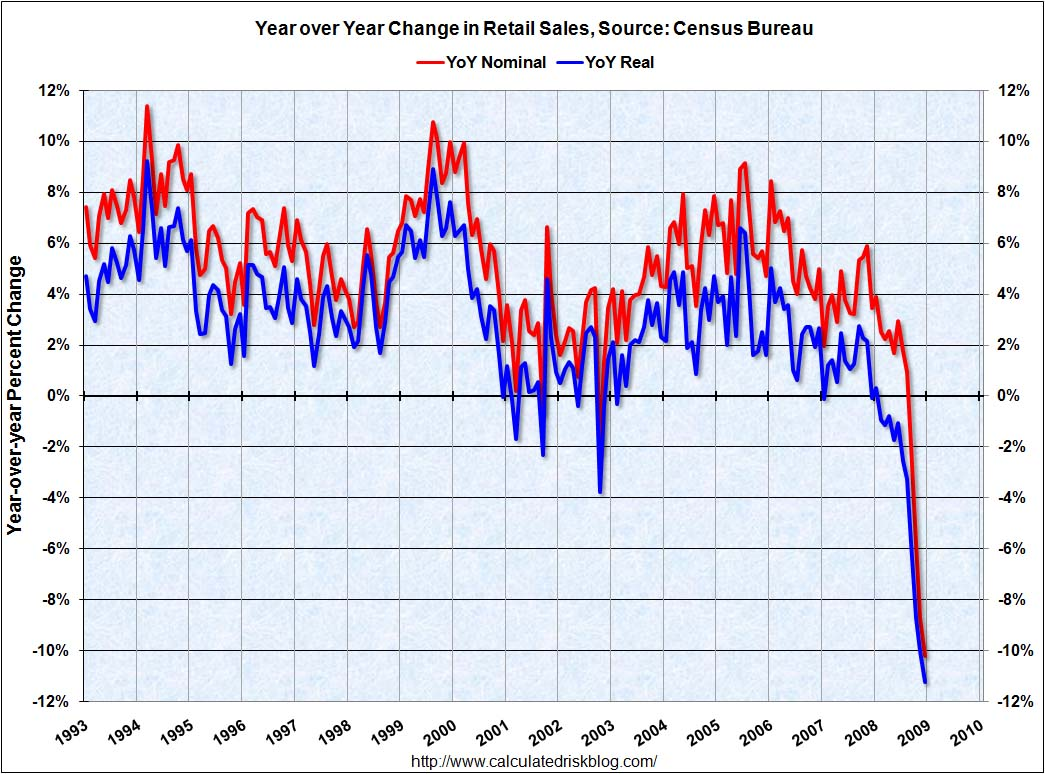
\includegraphics[width=2.5in]{/Volumes/Data/Job/Discuss/DiMaggio_Kermani/LaTeX/cfpbpresentation/Figures/Retail-Sales-Collapse.jpg}}
\end{center}

\end{frame}


\begin{frame}\frametitle{The Holy Grail}

\bi
\item A {\it reliable} (set of) {\it quantitatively useful} structural models
\bi
\item Theorists can 
\ei
\item What do we need?
\bi 
\item Much better {\it data and  {\bf models}} of expectations
\item Measures of {\it behavior conditional on expectations} ...
\item ... to be fed into a calibrated strucutural model
\ei
\ei

\end{frame}

\begin{frame}\frametitle{Wealth Effects (`Nexus')?}
\bi
\item ``Housing Wealth Effect'' estimates are converging
\item Kaplan, Mitman, Violante; Leth-Petersen and Andersen; CKHI
\item {\it Crucial} point: Size of effect depends on credit availability (`collateral channel')
\ei
\end{frame}


\begin{frame}\frametitle{Larry Summers' Infamous Quote about 2009-10}

{\it ``Almost nothing from the academic macroeconomics literature over the prior
30 years was useful in understanding what to do''} 

\begin{center}
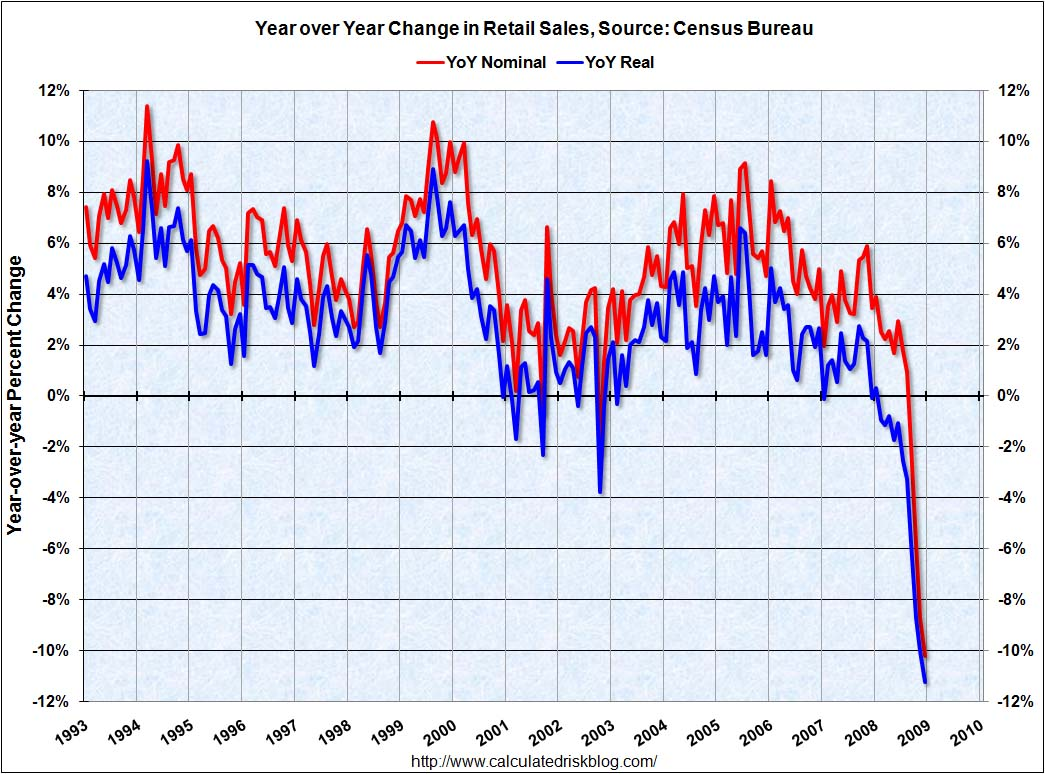
\includegraphics[width=2.5in]{/Volumes/Data/Job/Discuss/DiMaggio_Kermani/LaTeX/cfpbpresentation/Figures/Retail-Sales-Collapse.jpg}
\end{center}

\end{frame}

\begin{frame}\frametitle{Off-the-shelf Macro Models}

Zombies:
\bi
\item Rep Agent/Certainty Equivalent DSGE models
\item Campbell-Mankiw (Savers/Spenders) 
\ei

Desiderata: Uncertainty and Heterogeneity
\bi
\item Uncertainty
\bi
\item Landais \& Spinnewijn: Unemployment $\Rightarrow$ $C \downarrow$
\item $\Rightarrow$ uncertainty is hugely important
\ei
\item Heterogeneity
\bi
\item Concavity of the Consumption Function:
\bi
\item Low wealth people have much higher MPC's
\ei
\ei
\ei



\end{frame}

\begin{frame}\frametitle{Saving Over the Business Cycle}
\begin{center}
\includegraphics[width=3.0in]{/Volumes/Data/Papers/cssUSSaving/Latest/Figures/saving.pdf}
\end{center}
\end{frame}

\begin{frame}\frametitle{Unemployment Expectations $\Ex[\Delta \uLev_{t+1}]$}
\begin{center}
\includegraphics[width=3.0in]{/Volumes/Data/Papers/cssUSSaving/Latest/Figures/fUExp.pdf}
\end{center}
\end{frame}


\begin{frame}\frametitle{\cite{cssUSSaving}}

Model fit to aggregate saving rate history fits well.  Ranking of reasons for $s$ rise: \pause
\begin{itemize}
\item 60 percent: Uncertainty 
\bi
\item Michigan Survey: Unemployment Expectations
\ei
\item 25 percent: Wealth Effects
\item 15 percent: Credit Supply
\end{itemize}

\end{frame}

\begin{frame}\frametitle{National Registry Data}

Most important question they can answer:
\bi
\item {\it Whose} circumstances ($\yRat$, $\aRat$, etc) change
\item Whose {\it behavior} changes (`active saving')
\bi
\item Regional differences will be profoundly useful
\ei
\ei

\end{frame}

\begin{frame}\frametitle{High Frequency Data (Shapiro; Schuh)}

{\bf More is different:}
\bi
\item {\it Everything} is durable at the weekly frequency
\item Expenditure shocks can't be ignored
\item More `coping strategies' than we usually model
\ei

\end{frame}

\begin{frame}\frametitle{Surveys}

\begin{enumerate}
\item Survey design
\bi
\item Transaction, wealth, income data
\bi
\item Collect using technology (\texttt{Mint.com}, other aggregators)
\ei 
\item Only survey people on beliefs, expectations, preferences 
\ei
\item Use admin data as sampling frame for surveys
\bi
\item That way you get the combination
\ei
\bi
\item Need panel data on expectations to model them
\ei
\end{enumerate}

\end{frame}

\begin{frame}\frametitle{A New Day Is Dawning! }

\pause 
The scientific revolution is coming to macroeconomics!


\end{frame}


\end{verbatimwrite}
\input ./HeteroMacro-Slides-body.tex

\renewcommand{\bibsection}{\subsubsection*{\bibname }}

\nocite{denhaan:modelb}
\nocite{castaneda}


\beamerdefaultoverlayspecification{<*>}

\begin{frame}[t,allowframebreaks]
\frametitle{References}
\tiny 
\input econtexBibMake
\end{frame}
\pagebreak

\end{document}

\begin{frame}
\includegraphics[width=3.0in]{/Volumes/Data/Work/EpidemiologyOfMacro/DataAndPrograms/Data/inflstd}
\end{frame}

\begin{frame}
\includegraphics[width=3.0in]{"/Volumes/Data/Work/A Theory of the ConsFunc/A Theory ... Draft 3/STATA/scfcdf"}
\end{frame}

